
\chapter{Data Cloud and Cloud Security}

\section{Data Cloud}

\textbf{Cloud Storage} is a service model in which data is maintained, managed and backed up remotely and made available to users over a network (typically the Internet). Users generally pay for their cloud data storage on a per-consumption, monthly rate. Although the per-gigabyte cost has been radically driven down, cloud storage providers have added operating expenses that can make the technology more expensive than users bargained for. Cloud security continues to be a concern among users. Providers have tried to address those fears by building security capabilities, such as encryption and authentication, into their services.

Traditional storages are:

\begin{minipage}{0.45\textwidth}
    \textbf{Block Storage}:
    \begin{itemize}
        \item Volumes
        \item Blocks (read/write)
        \item Fibre Channel or iSCSI protocols
        \item Local
        \item Low latency, high IOPs, low size (<1PB)
        \item Complex to expand and expensive 
    \end{itemize}
\end{minipage}
\begin{minipage}{0.45\textwidth}
    \begin{figure}[H]
        \centering
        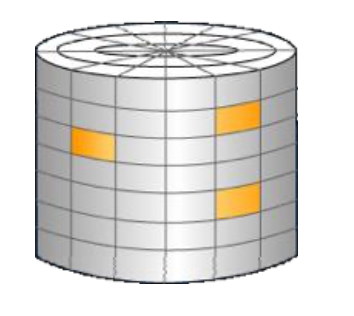
\includegraphics[width=0.5\textwidth]{assets/fig40.png}
        \caption{Block Storage}
    \end{figure}
\end{minipage}

\begin{minipage}{0.45\textwidth}
    \begin{figure}[H]
        \centering
        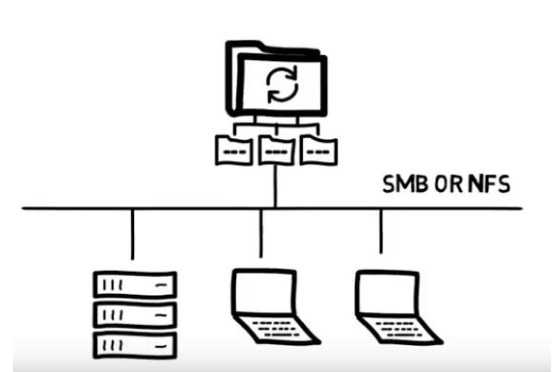
\includegraphics[width=0.7\textwidth]{assets/fig41.png}
        \caption{File Storage}
    \end{figure}
\end{minipage}
\begin{minipage}{0.45\textwidth}
    \textbf{File Storage}:
    \begin{itemize}
        \item Files
        \item NFS, SMB, FTP, etc.
        \item Local
        \item Low latency, high IOPs, low size (<1PB)
        \item Complex to expand and expensive 
    \end{itemize}
\end{minipage}

\subsection{Distributed File System}

\begin{definitionblock}[Distributed File System]
    A \textbf{Distributed File System} is a shared file system that allows many clients to access files and directories stored on a central server. It is a client/server-based application that allows clients to access and process data stored on the server as if it were on their own computer.

    \begin{itemize}
        \item \textbf{Client}: The client is the end-user device that accesses the files stored on the server.
        \item \textbf{Server}: The server is the computer that stores the files and directories that the clients access.
    \end{itemize}
\end{definitionblock}

Properties:
\begin{itemize}
    \item \textbf{Transparency}: A client cannot tell where a file is located. A file can transparently move to another server. Multiple copies of a file may exist. Multiple clients access the same file.
    \item \textbf{Flexibility}: Servers may be added or replaced and there is support for multiple file system types.
    \item \textbf{Dependability}: Conflicts with replication and concurrency control. Users may have different access rights on clients sharing files and network transmission. Server crashes may cause data loss.
    \item \textbf{Performance}: Requests may be distributed across servers and multiple servers allow higher storace capacity.
    \item \textbf{Caching}: Reduce network traffic by retaining recently accessed disk blocks in a cache, so that repeated accesses to the same information can be handled locally. If required data is not already cached, a copy of data is brought from the server to the user. 
\end{itemize}

Configuration and implementation may vary, servers may run on dedicated machines or servers and clients can be on the same machines. 

\begin{figure}[H]
    \centering
    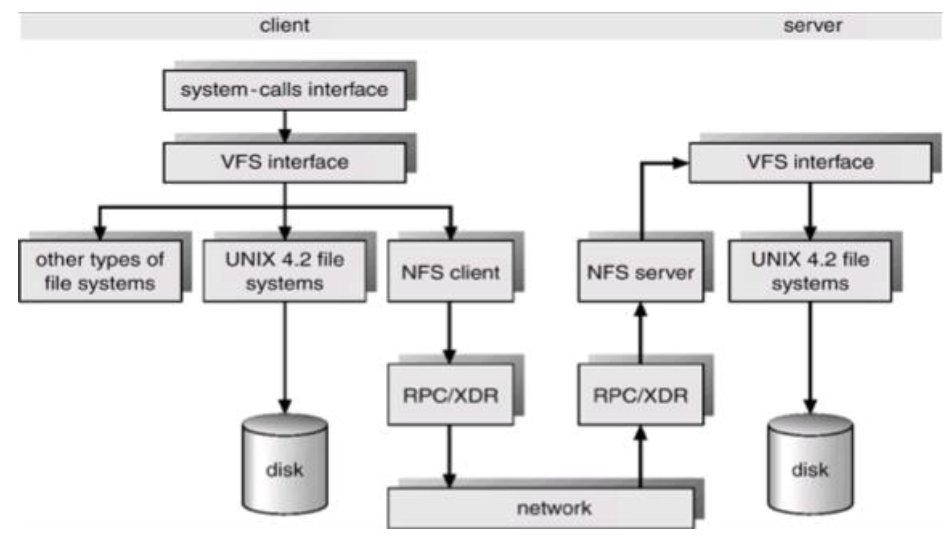
\includegraphics[width=0.7\textwidth]{assets/fig42.png}
    \caption{Distributed File System}
\end{figure}

\begin{warningblock}[Limitations of traditional storage]
    Traditional storage systems are limited in terms of scalability, performance, and cost. They are not designed to handle the massive amounts of data that are generated by modern applications. They are also not designed to handle the high levels of concurrency that are required by modern applications. In addition, traditional storage systems are expensive to purchase and maintain. They require a significant amount of hardware and software to be installed and configured, and they require a dedicated team of IT professionals to manage them.
\end{warningblock}

\begin{exampleblock}[Google File System]
    The Google File System (GFS) is a distributed file system that was developed by Google to handle the massive amounts of data that are generated by its search engine. GFS is designed to be highly scalable, highly available, and highly reliable. It is designed to handle the high levels of concurrency that are required by modern applications. GFS is also designed to be cost-effective, with a low total cost of ownership. GFS is based on a master/slave architecture, with a single master server that manages the metadata for the file system and multiple slave servers that store the actual data. GFS uses a distributed lock service to manage access to the file system, and it uses a distributed file system protocol to communicate between the master and slave servers. GFS is designed to be fault-tolerant, with multiple copies of each file stored on different servers to ensure that data is not lost in the event of a server failure. GFS is also designed to be highly available, with multiple master servers that can take over in the event of a master server failure. GFS is designed to be highly reliable, with built-in mechanisms for detecting and recovering from data corruption and other errors.

    \begin{itemize}
        \item \textbf{Master Server}: Single master server that manages the metadata for the file system.
        \item \textbf{Chunk Servers}: Multiple slave servers that store the actual data.
    \end{itemize}
    
    \begin{figure}[H]
        \centering
        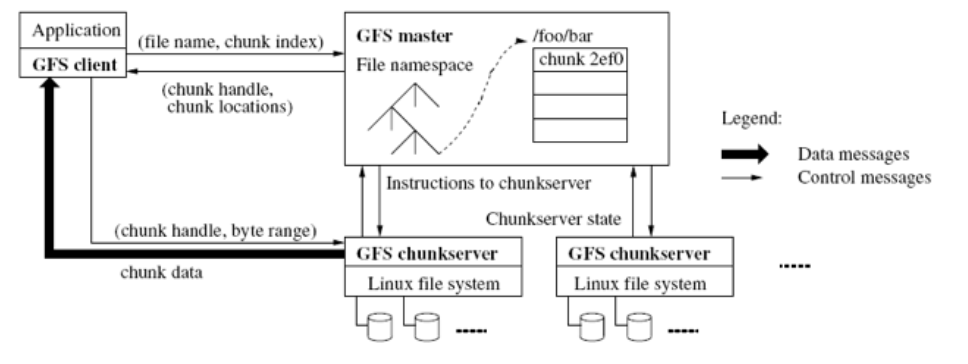
\includegraphics[width=0.7\textwidth]{assets/fig43.png}
        \caption{Google File System Architecture}
    \end{figure}

    \begin{figure}[H]
        \centering
        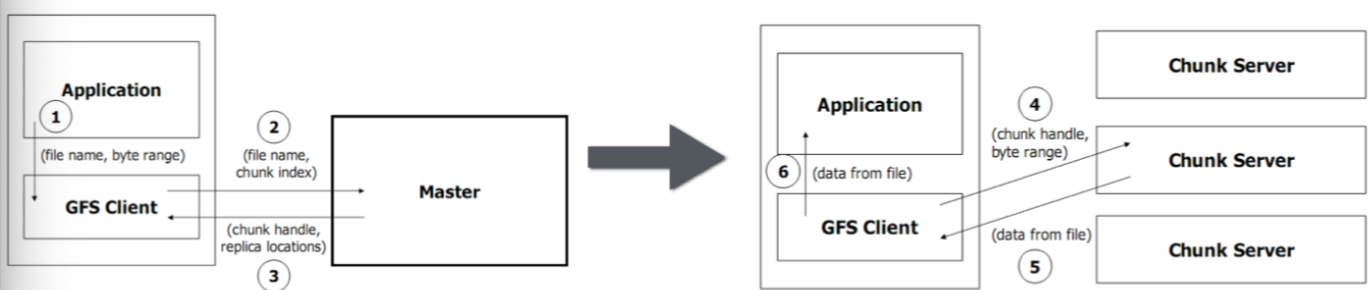
\includegraphics[width=0.9\textwidth]{assets/fig44.png}
        \caption{Read Files}
    \end{figure}
\end{exampleblock}

An \textbf{object} is a logical unit of storage that is stored on a server. An object has a unique identifier, a set of attributes, and a set of methods that can be used to access and manipulate the object. Objects are typically stored in a distributed file system, where they are replicated across multiple servers to ensure high availability and durability. Objects are typically accessed using a RESTful API, which allows clients to perform CRUD operations on the objects using standard HTTP methods.

\textbf{Metadata}, instead, is data that describes the attributes of an object. Metadata is typically stored in a separate database or file system from the object itself, and is used to store information such as the object's name, size, type, and location. Metadata is typically accessed using a separate API from the object itself, which allows clients to query and update the metadata without having to access the object itself.

\begin{observationblock}[FITS files]
    The Flexible Image Transport System (FITS) is an open standard defining a digital file format useful for storage, transmission and processing of data: formatted as multi-dimensional arrays (images) or tables. FITS is the most commonly used digital file format in astronomy. FITS is much more than just another image format (such as JPG or GIF) and is primarily designed to store scientific data sets consisting of multi-dimensional arrays (2D tables, 3D data cubes, etc.) and 1D tables consisting of columns and rows. FITS is also often used to store non-image data, such as spectra, photon lists, data cubes, or structured data such as object catalogs.
\end{observationblock}

Request for storage are made with HTTP using RESTful APIs. The request is made to the server, which is responsible for storing the data. The server then stores the data in a distributed file system, which replicates the data across multiple servers to ensure high availability and durability. The server then returns a response to the client, which indicates whether the request was successful or not. Primary components of a request are:
\begin{enumerate}
    \item HTTP Verb: GET, POST, PUT, DELETE
    \item Authentication Information 
    \item SURL: Storage URL
    \item Metadata (optional)
\end{enumerate}

\begin{figure}[H]
    \centering
    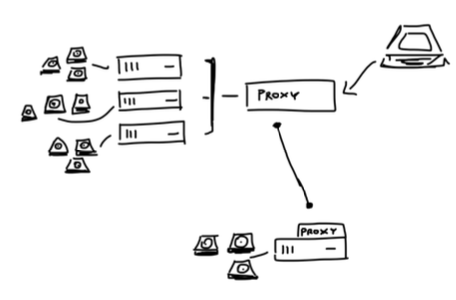
\includegraphics[width=0.7\textwidth]{assets/fig45.png}
    \caption{Request for Storage}
\end{figure}

\begin{figure}[H]
    \centering
    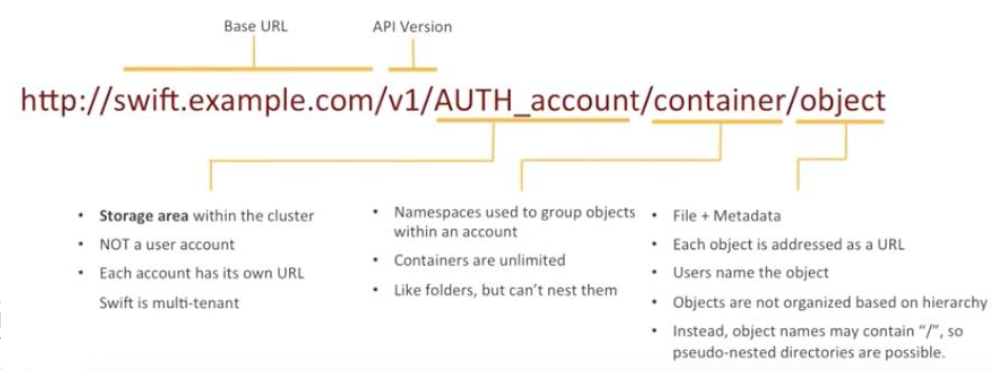
\includegraphics[width=0.9\textwidth]{assets/fig46.png}
    \caption{manage Object with HTTP}
\end{figure}

\subsection{Cloud Storage capabilities}

\begin{definitionblock}[Cloud Storage]
    \textbf{Cloud Storage} is a service model in which data is maintained, managed and backed up remotely and made available to users over a network (typically the Internet). Users generally pay for their cloud data storage on a per-consumption, monthly rate. Although the per-gigabyte cost has been radically driven down, cloud storage providers have added operating expenses that can make the technology more expensive than users bargained for. Cloud security continues to be a concern among users. Providers have tried to address those fears by building security capabilities, such as encryption and authentication, into their services.
\end{definitionblock}

Its capabilities are:
\begin{itemize}
    \item \textbf{Cloud File Storage}: Store and manage files in the cloud. Files are stored in a distributed file system, which replicates the data across multiple servers to ensure high availability and durability. Files are typically accessed using a RESTful API, which allows clients to perform CRUD operations on the files using standard HTTP methods.
    \item \textbf{User management}: Manage users and their access to files. Users are typically authenticated using a username and password, and their access to files is controlled using access control lists (ACLs). Users can be assigned different roles and permissions, which determine what actions they can perform on the files.
    \item \textbf{Easy to use GUI}: A graphical user interface (GUI) that allows users to easily upload, download, and manage files in the cloud. The GUI typically provides a file browser that allows users to navigate the file system, and a set of buttons that allow users to perform common file operations.
    \item \textbf{Security}: Security features such as encryption, authentication, and access control. Files are typically encrypted at rest and in transit, to protect them from unauthorized access. Users are authenticated using a username and password, and their access to files is controlled using access control lists (ACLs).
    \item \textbf{Scalability}: Scalability features such as automatic scaling and load balancing. The cloud storage system is designed to automatically scale to handle large amounts of data and high levels of concurrency. Load balancing ensures that requests are distributed evenly across the servers, to prevent any one server from becoming overloaded.
    \item \textbf{Multiple access protocols}: Support for multiple access protocols, such as RESTful APIs, NFS, and SMB. Users can access files using a variety of protocols, depending on their needs and preferences. RESTful APIs are typically used for programmatic access, while NFS and SMB are typically used for file sharing and collaboration.
\end{itemize}

Its architecture is based on a distributed file system, which replicates the data across multiple servers to ensure high availability and durability. The distributed file system is typically accessed using a RESTful API, which allows clients to perform CRUD operations on the files using standard HTTP methods. The distributed file system is typically implemented using a master/slave architecture, with a single master server that manages the metadata for the file system and multiple slave servers that store the actual data.

\begin{figure}[H]
    \centering
    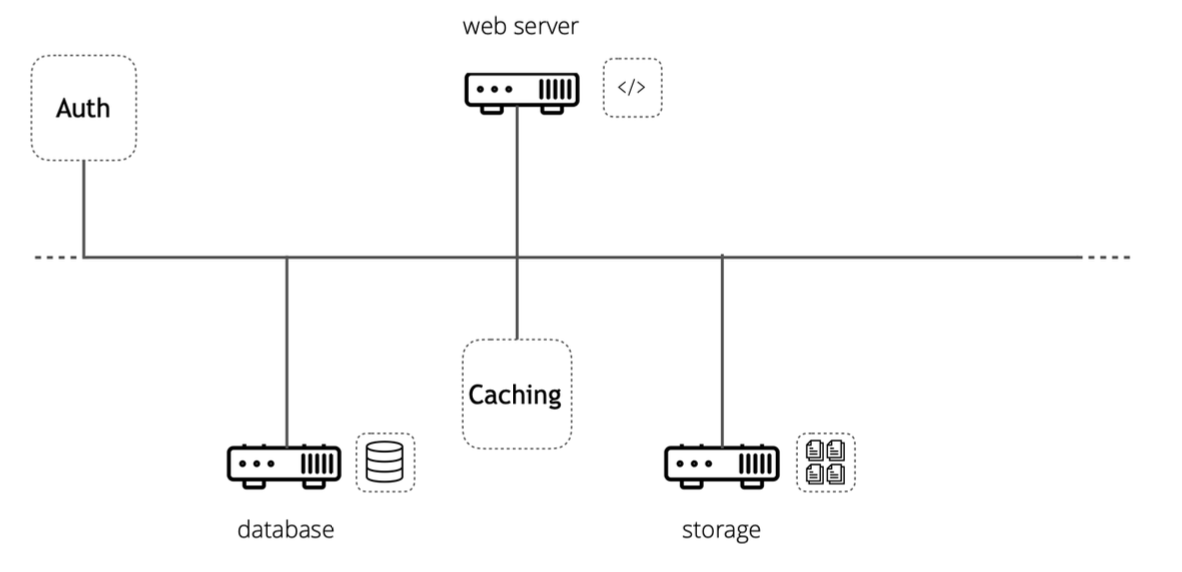
\includegraphics[width=0.9\textwidth]{assets/fig47.png}
    \caption{Cloud Storage Architecture}
\end{figure}

\begin{figure}[H]
    \centering
    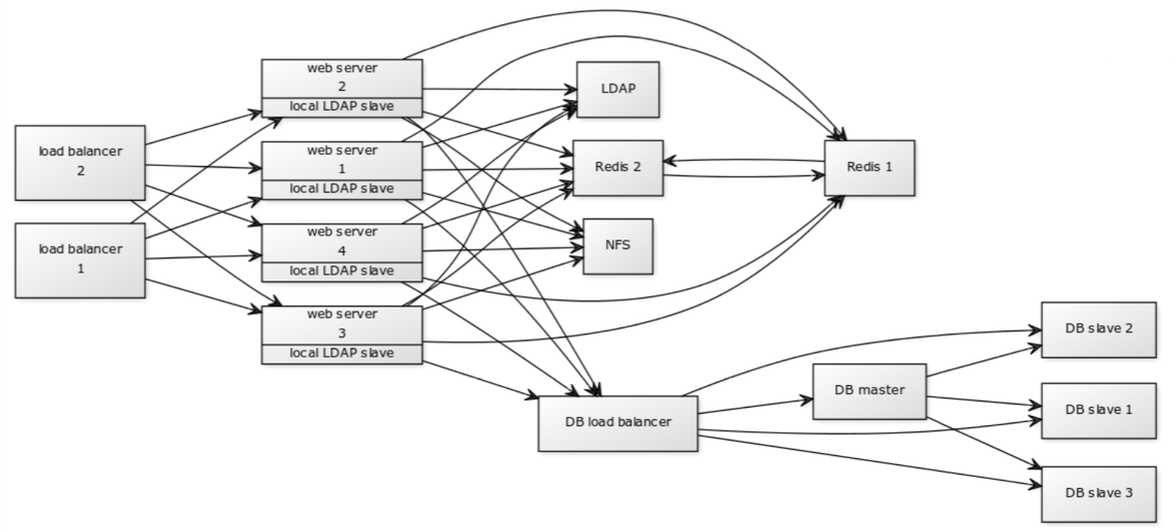
\includegraphics[width=0.9\textwidth]{assets/fig48.png}
    \caption{Production Deployment}
\end{figure}

To \textbf{monitor} the system several tools can be used:
\begin{itemize}
    \item \textbf{Docker stats}: Command line tool that provides real-time resource usage statistics for Docker containers.
    \item \textbf{Portainer}: Management tool for Docker environments, easy to setup.
    \item \textbf{Grafana}: Analytics and visualization platform that allows users to query, visualize and monitor data from multiple sources in real-time. Requires configuration. 
\end{itemize}

\section{Cloud Security}

\begin{figure}[H]
    \centering
    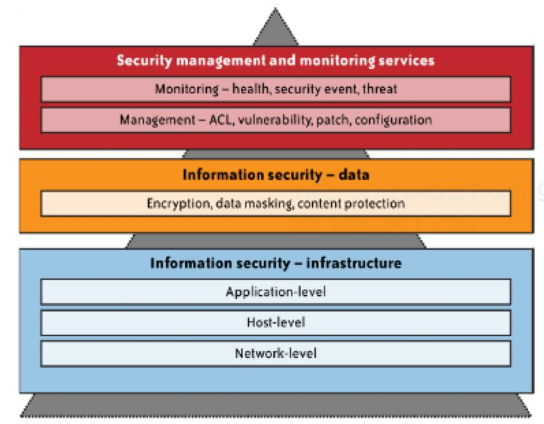
\includegraphics[width=0.6\textwidth]{assets/fig49.png}
    \caption{Cloud Security}
\end{figure}

Different types of cloud computing service models provide different levels of security. There are three levels of cloud security:
\begin{itemize}
    \item \textbf{Network Level}: Security at the network level is the most basic level of security. It involves securing the network infrastructure that connects the cloud servers to the Internet. This includes firewalls, intrusion detection systems, and other network security devices. Network security is important because it protects the cloud servers from attacks that originate from the Internet.
    \item \textbf{Host Level}: Security at the host level is the next level of security. It involves securing the individual servers that make up the cloud infrastructure. This includes securing the operating system, the applications that run on the server, and the data that is stored on the server. Host security is important because it protects the cloud servers from attacks that originate from within the cloud infrastructure.
    \item \textbf{Application Level}: Security at the application level is the highest level of security. It involves securing the applications that run on the cloud servers. This includes securing the code that makes up the application, the data that the application processes, and the users that access the application. Application security is important because it protects the cloud servers from attacks that exploit vulnerabilities in the application code.
\end{itemize}

So, before approaching the cloud, it is important to understand the security risks and challenges that come with it. The most common security risks and challenges associated with cloud computing are:
\begin{itemize}
    \item \textbf{Data Breaches}: Data breaches are one of the most common security risks associated with cloud computing. A data breach occurs when an unauthorized party gains access to sensitive data stored in the cloud. This can happen through a variety of means, such as hacking, phishing, or social engineering.
    \item \textbf{Data Loss}: Data loss is another common security risk associated with cloud computing. Data loss occurs when data stored in the cloud is accidentally deleted, corrupted, or otherwise lost. This can happen due to a variety of reasons, such as hardware failure, software bugs, or human error.
    \item \textbf{Account Hijacking}: Account hijacking is a security risk that occurs when an unauthorized party gains access to a user's cloud account. This can happen through a variety of means, such as phishing, social engineering, or weak passwords. Once an attacker gains access to a user's account, they can steal sensitive data, delete files, or perform other malicious activities.
    \item \textbf{Insecure APIs}: Insecure APIs are a security risk that occurs when the APIs used to access cloud services are not properly secured. This can happen due to a variety of reasons, such as weak authentication mechanisms, lack of encryption, or other vulnerabilities in the API implementation. Insecure APIs can be exploited by attackers to gain unauthorized access to sensitive data or perform other malicious activities.
    \item \textbf{Insider Threats}: Insider threats are a security risk that occurs when an authorized user of a cloud service intentionally or unintentionally causes harm to the service. This can happen due to a variety of reasons, such as disgruntled employees, careless users, or users who are tricked by attackers. Insider threats can be difficult to detect and prevent, as the attacker already has legitimate access to the service.
\end{itemize}

\subsection*{Host Level}

\begin{itemize}
    \item \textbf{Hypervisor security}: The hypervisor is a critical component of the cloud infrastructure, as it is responsible for managing the virtual machines that run on the physical servers. Hypervisor security is important because a compromise of the hypervisor can lead to a compromise of all the virtual machines that run on it. Hypervisor security can be improved by using secure hypervisors, keeping the hypervisor up to date, and using strong access controls.
    \item \textbf{Virtual Machines security}: Virtual machines are the building blocks of the cloud infrastructure, as they run the applications that make up the cloud services. Virtual machine security is important because a compromise of a virtual machine can lead to a compromise of the data and applications that run on it. Virtual machine security can be improved by using secure virtual machine images, keeping the virtual machines up to date, and using strong access controls. Also ssh keys can be used to access the virtual machines.
\end{itemize}

The VM/Containers security has the advantages of a simpler implementation of resource management policies, along with improved intrusion prevention and detection and more efficient software testing. 

The OS implement minimal security on: Access control, authentication usage and cryptographic usage policies. Applications with special privilegies that perform security-related functions are called trusted applications. They should only be allowed in the lowest level of privileges required to perform their functions. An OS poorly isolates one application from another, and once an application is
compromised, the entire physical platform and all applications running on it can be
affected.

For \textbf{Data Security}, Identify the security boundary separating the client’s and vendor’s responsibilities
Determine the sensitivity of the data to risk
Data should be transferred and stored in an encrypted format.
Separate clients from direct access to shared cloud storage.

The following are the mechanism for protecting data:
\begin{itemize}
    \item \textbf{Access control}, which is the process of determining who can access what data and under what conditions. Access control is typically implemented using a combination of authentication, authorization, and auditing mechanisms.
    \item \textbf{Auditing}, which is the process of monitoring and recording access to data. Auditing is typically implemented using a combination of logging, monitoring, and reporting mechanisms.
    \item \textbf{Authentication}, which is the process of verifying the identity of a user. Authentication is typically implemented using a combination of passwords, biometrics, and other authentication mechanisms.
    \item \textbf{Authorization}, which is the process of determining what data a user can access. Authorization is typically implemented using a combination of access control lists, role-based access control, and other authorization mechanisms.
\end{itemize}

You should isolate data from direct client access, creating a layered access to it. Use data segregation based on tenants.

\begin{figure}[H]
    \centering
    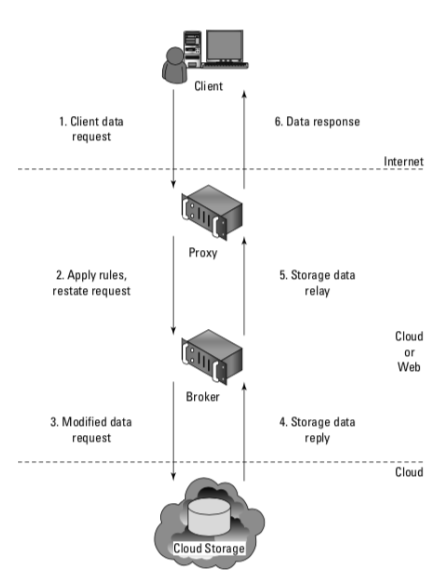
\includegraphics[width=0.5\textwidth]{assets/fig50.png}
    \caption{Data Security}
\end{figure}

Most clooud service providers store data in an encrypted form on server side or client side. 

Problems:
\begin{itemize}
    \item a problem with encrypted data may result with data that may not be
    recoverable.
    \item it does nothing to prevent data loss: keep your keys!
\end{itemize}




